\label{chap:machine_learning}

%%% BOZZA %%% % ESTIMATE 1h

Il workflow del machine learning è produrre dei modelli di machine learning
addestrati sui dati che possono. Prima di parlare di come si crea e che
modelli di machine learning andremo a creare, parleremo di come automatizzare
la creazione di questi modelli. 
However, the real challenge isn't building an ML model, the
challenge is building an integrated ML system and to continuously operate it
in production.

create

In questo capitolo prima di parlare degli algoritmi di Machine Learning utilizzati,
spiegheremo come arrivare a poter ottenere un modello, e ciò verrà affatto
attraverso la creazione di una pipeline.

Una pipeline consiste in una sequenza di più step indipendenti che sono
linkati tra di loro per risolvere un task. Le pipeline nel machine learning
consistono in step multipli sequenziali che fanno tutto da estrarre i dati a
preprocessarli per l'addestramento del modello, al deployment e la sua
valutazione. Possiamo vedere una pipeline come un DAG (Directed Acyclic
Graph), dove i dati fluiscono in un solo senso. Acyclic perché non sono
permessi loop e dove ogni nodo corrisponde a uno step di Machine Learning

The four main steps in an ML pipeline are data preparation, model training, model deployment,

linkando insieme diversi step insieme noi possiamo automatizzare il workflow
che serve per produrre un modello di Machine Learning. Ciò è importante,
perché se pensiamo di avere tanti step di trasformazioni, e a ogni set di dati
che utilizziamo bisogna applicare le stesse trasformazioni, avendo incapsulato
in un'unica entità che utilizziamo possiamo salvare tempo e effort.

Rapid experiment: The steps of the ML experiment are orchestrated. The
transition between steps is automated, which leads to rapid iteration of
experiments and better readiness to move the whole pipeline to production.

Modularized code for components and pipelines: To construct ML pipelines,
components need to be reusable, composable, and potentially shareable across
ML pipelines. Therefore, while the EDA code can still live in notebooks, the
source code for components must be modularized. I

Nelle prossime sezioni parleremo di tutti gli step legati all'estrazione dei
dati, alla loro Preprocessing, al model building, e come in ogni step è stato
osservato come poter integrare 

Nelle prossime sezioni parleremo di tutti gli step legati a un workflow di
machine learning e di come è stato osservato un occhio di riguardo rispetto
alla produzione della pipeline.

Ometteremo solo di trattare lo step iniziale del Data collection, ovvero
raccogliere i dati grezzi da diverse fonti di dati e immagazzinarle, poiché
è stato parte del lavoro iniziale del Dott. Stefano Dal Pra che tramite un cron e
diversi script ha collezionato i dati grezzi dalle diverse fonti come dai file history 
Stefano Dal Pra e del monitoraggio dei job da HtCondor e non  riguarda questa
trattazione.

% in più è possibile ottimizzare la pipeline tutta insieme e ricercare gli
% iperaparametri migliori, breve spiegazione sui parametri e iperaparametri

%%% FINE BOZZA %%%

\section{Estrazione dei dati} % ESTIMATE 1h

%%% BOZZA %%%



%%% FINE BOZZA %%%

Data extraction: You select and integrate the relevant data from various data sources for the ML task.
We cannot directly input the collected data to train the model without pr-processing it, as it may generate an abrupt result.

Procediamo con l'estrazione di un dataset tramite la query SQL che
interroga le tabelle \texttt{hj} e \texttt{htjob}. Ricordando che:
\begin{itemize}
    \item La tabella \texttt{hj} contiene lo stato dei job, rappresentato da
        serie storiche di misurazioni (come \texttt{runtime}, \texttt{ram},
        \texttt{swap}, \texttt{disk}, ecc.),
        durante la loro esecuzione.
    \item La tabella \texttt{htjob} fornisce informazioni sull'esito dei job,
        ovvero se sono falliti o meno.
\end{itemize}

% fail 
% jobid.idx.submitnode

La query esegue le seguenti operazioni:
\begin{itemize}
    \item Seleziona i job che hanno iniziato e finito la loro esecuzione nel
        periodo temporale specificato.
    \item Esegue un JOIN delle tabelle utilizzando l'identificativo univoco di
        ciascun job (\textit{jobid.idx\_submitnode}) e il timestamp. Questo
        timestamp sfrutta l'indice presente nella tabella
        \texttt{hj} per gestire in maniera efficiente le grandi dimensioni di
        questa tabella\footnote{La logica dietro questo consiste
            nel selezionare un job da \texttt{htjob} e successivamente
            cercarlo in \texttt{hj} limitando la ricerca ai record che
            rientrano nel periodo in cui \texttt{hj.ts} è compreso tra
            \texttt{htjob.starttimeepoch} e \texttt{htjob.eventtimeepoch}.
            Questo permette di restringere notevolmente la ricerca nella
            tabella \texttt{hj} per ogni job selezionato da \texttt{htjob} ed
        evitare di scansionare l'intera tabella.}. Poiché la tabella \texttt{hj} contiene più record per
        ogni job, la query li raggruppa per job. In seguito, mediante l'uso
        dell'operatore \verb|ARRAY_AGG|, le serie storiche vengono trasformate
        in liste di valori.
    \item Filtra i job con un tempo di esecuzione superiore a un'ora
        (\verb|runtime > 3600|), in quanto i job più brevi sono considerati
        irrilevanti per lo scopo dello studio.
\end{itemize}

Il risultato di questa query è un dataset come mostrato nella
figura~\ref{fig:dataset_from_join_hj_htjob}, dove ogni riga rappresenta un job
e le colonne includono: 

\begin{itemize}
    \item \texttt{job}: identificativo univoco per ogni job.
    \item \texttt{queue}: gruppo di appartenenza dell'utente che ha sottomesso
        il job.
    \item \texttt{fail}: una variabile booleana che indica se il job è fallito.
    \item \texttt{mint} e \texttt{maxt}: il tempo minimo e massimo di
        esecuzione del job.
    \item \texttt{t}, \texttt{ram}, \texttt{swap}, \texttt{disk}: liste di
        valori che rappresentano le serie storiche di misurazioni.
\end{itemize}

Il dataset ottenuto comunque non è sufficiente per poter applicare
direttamente un algoritmo di Machine Learning, infatti le colonne che
rappresentano le serie storiche univariate contengono un tipo di dato
complesso, come delle liste. Questo ha bisogno di essere preprocessato e
aggiungere ulteriori informazioni che si possono astrarre dai dati e rendere i
dati utilizzabili da un algoritmo. Dobbiamo risolvere tutti i problemi
spiegati nella sezione delle serie storiche \ref{}.

% che cos'è un DataFrame

\begin{figure}
    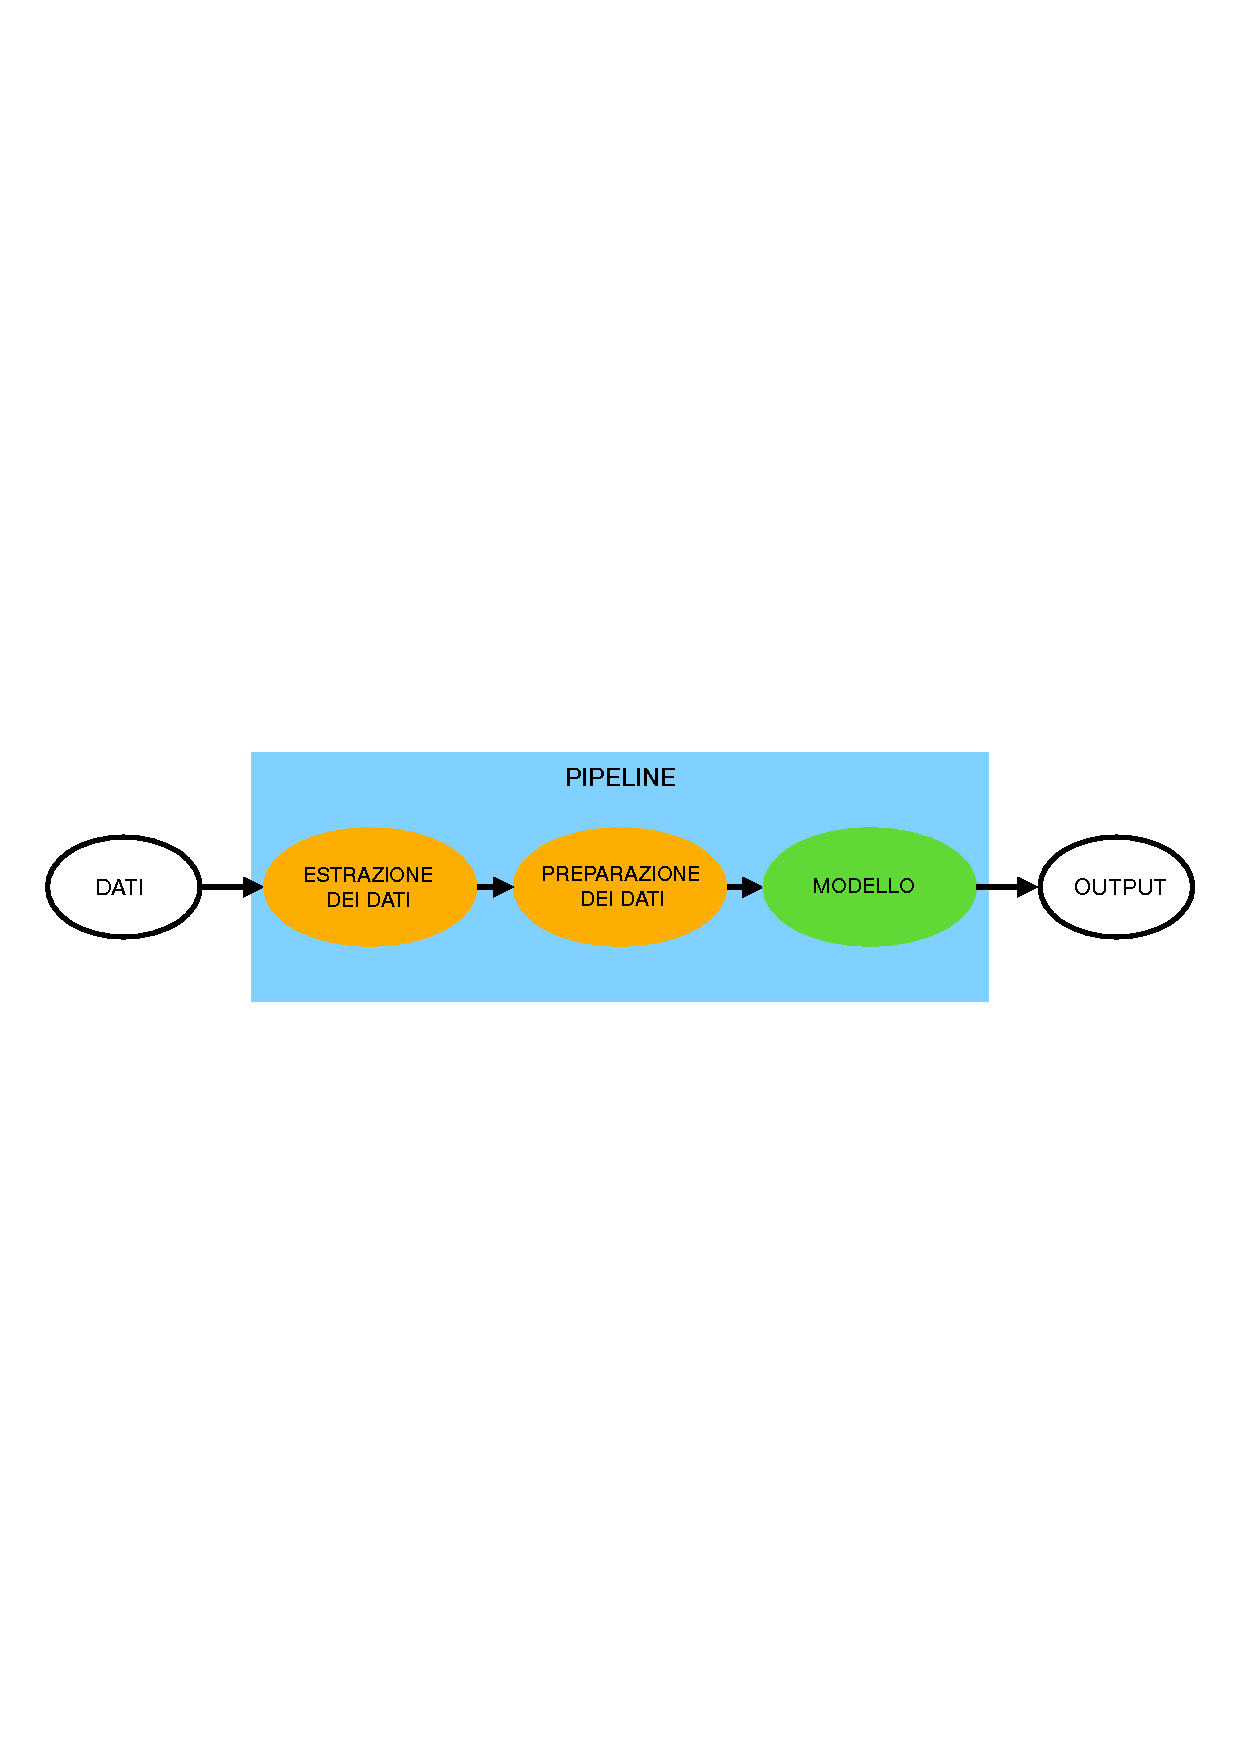
\includegraphics[trim=0 13cm 0 13cm, clip, width=\linewidth]{pipeline}
    \caption{}
    \label{}
\end{figure}

\begin{figure}[!ht]
    \centering
    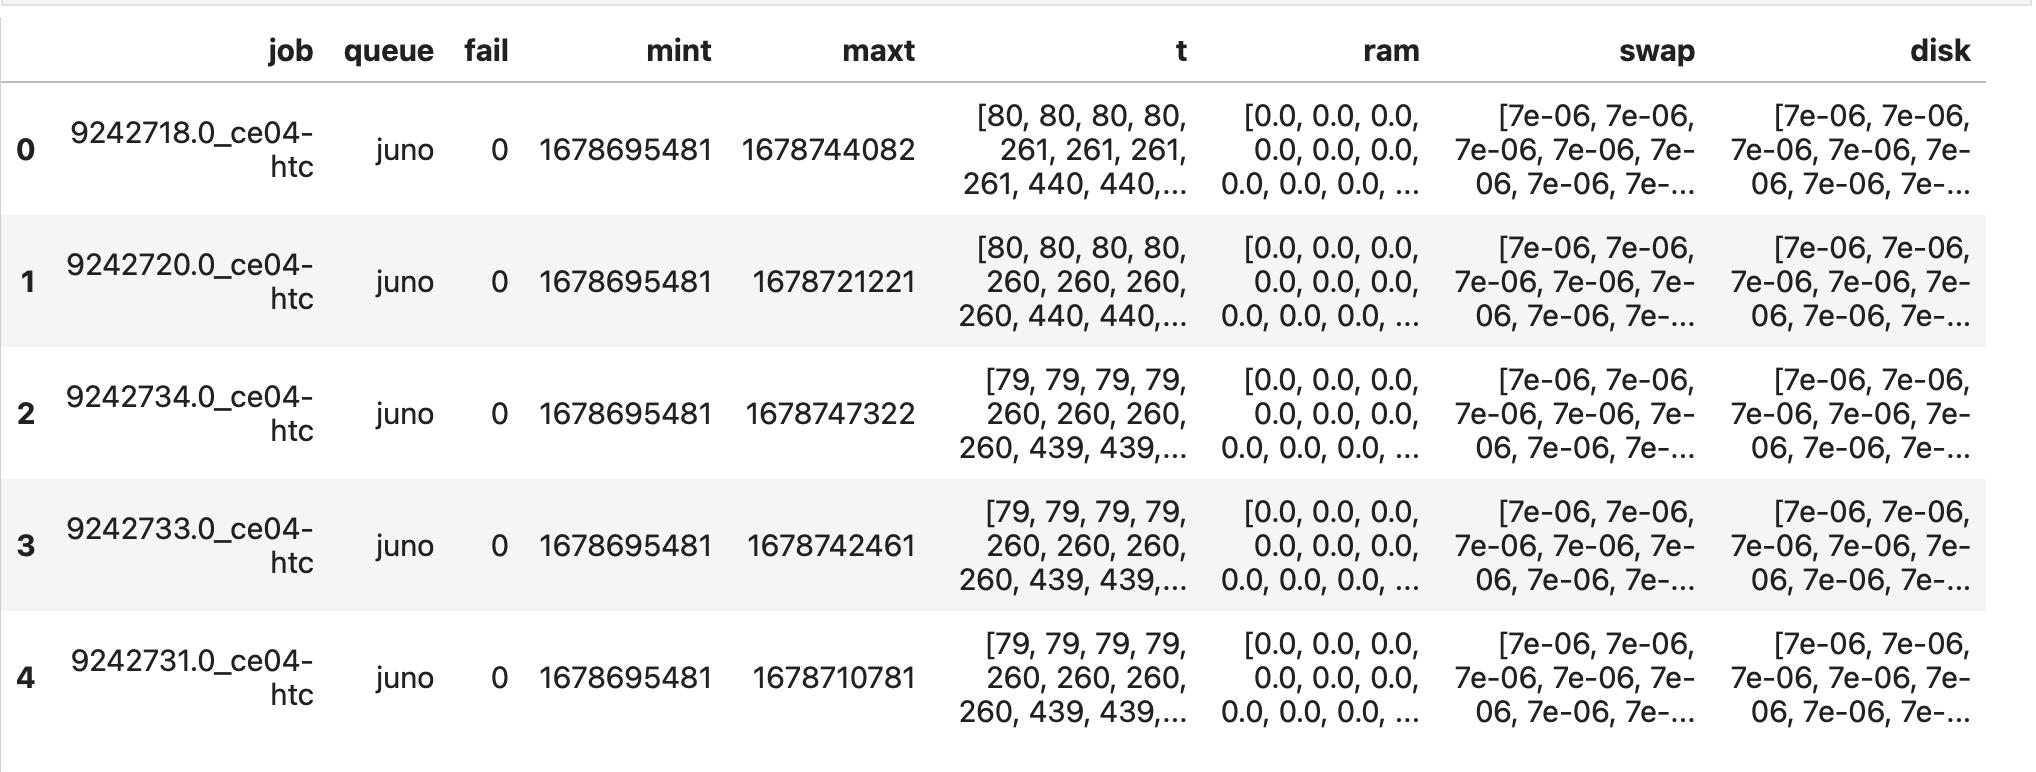
\includegraphics[width=0.95\textwidth]{dataset}
    \caption{Le prime cinque righe del dataset}
    \label{fig:dataset_from_join_hj_htjob}
\end{figure}

\section{Preparazione dei dati} % ESTIMATE 13h


%%% BOZZA 
I dati vengono preparati per il task di machine learning

Gli algoritmi di Machine Learning richiedono che i dati siano dei numeri.

Inoltre,
Se la qualità o la quantità dei dati sono insufficienti, noi andremo incontro
a una situazione comunemente chiamata ``garbage in, garbage out'' e non
importa quanto sia figo il nostro algoritmo di machine learning, perché non
avremo risultati soddisfacenti. Infatti più è fancier l'algoritmo, più dati
avremo bisogno.

Data l'esistenza di dati di bassa qualità, per aumentare la qualità del
modello che vogliamo utilizzare, i dati DEVONO ESSERE PREPARATI.

% rimozione rumore
Rumore nei dati e errori possono essere corretti
Complex nonlinear relationships may be teased out of the data.
 r how to best expose the underlying structure of the problem to the learning algorithms. This is the guiding light.

Le tecniche di pre-processing si riferiscono generalmente all'addition,
deletion o la trasformazione dei dati iniziali 

%%% FINE BOZZA %%%

%In questa tesi considereremo un Preprocessor come un algoritmo che prende un
%DataFrame e restituisce un altro DataFrame, applicando una serie di passaggi
%intermedi

% Transformer is an algorithm which can transform one DataFrame into another DataFrame

%Data preparation: The data is prepared for the ML task. This preparation
%involves data cleaning. You also apply data transformations and feature engineering to
%the model that solves the target task. The output of this step are the data

% qua parleremo del preprocessor

% template method

 % costruendo un componente così fatto per la pipeline possiamo ricercare gli
% iperaparametri migliori di ciascuna trasformazione fatta

\subsection{Trasformazione delle serie storiche multivariate multiple} %
% ESTIMATE 5h

% dobbiamo convertire le serie storiche in un tipo di dati strutturato,
% tabellare, utilizzabile dai modelli di Machine Learning

% padding e truncate delle serie storiche 

% avg pooling

% tabular transformation

% tensor transformation

\subsection{Creazione delle feature} % ESTIMATE 2h
\begin{figure}[!ht]
    \centering
    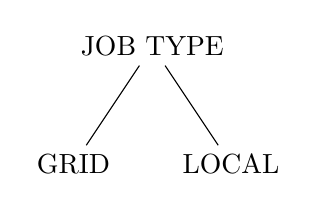
\begin{tikzpicture}[sibling distance=2cm]
        \node {JOB TYPE}
            child {node {GRID}}
            child {node {LOCAL}};
    \end{tikzpicture}
    \hspace{2cm}
    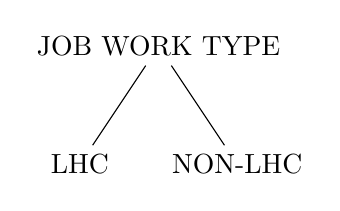
\begin{tikzpicture}[sibling distance=2cm]
        \node {JOB WORK TYPE}
        child {node {LHC}}
        child {node {NON-LHC}};
    \end{tikzpicture}
\end{figure}

% non contiene dati duplicati e missing values

% Data preparation: The data is prepared for the ML task. This preparation

% jobid e idx

% jobid e idx sono creati dal Submit Node al "concepimento" del job (es.
% 'sn-01', 'ce03-htc', ...). I S.N. sono indipendenti tra loro per cui in linea
% di principio possono esistere due job diversi con (jobid,idx) uguale (in tal
% caso vengono da S.N. diversi)%

% job work type

% job type

% one hot encoding 

% non verranno considerati i jobs con runtime <
% 1h, poichè non rilevanti per il sistema.

% variabili categoriche
% queue
% one hot encoding
%
% your system will only be capable of learning if the training data enough
% relevant and not too many irrilevant ones. A critical part of the success of
% a machine learning project is coming up with a good set of features to train
% on.
% This process, called feature engineering

\subsection{Etichettatura dei dati} % ESTIMATE 1h

% Una possibile strategia:
% - usando htjob si trovano i job eliminati per "toomuchtime": sono quelli con
%   jobstatus = 3 e runtime ~=7gg (non c'è valore esatto!)
% - a questo punto possiamo possiamo impostare un supervised learning
%   guardando su hj come hanno "vissuto" quei job.

\subsection{Tecniche di bilanciamento dei dati} % ESTIMATE 5h

% undersample

% oversample

% class weighting in loss function

% Metriche

\section{Selezioni dei modelli}
\subsection{Modelli supervisionati}
\subsection{Modelli non supervisionati}
\section{Valutazione delle performance}
\subsection{Metriche di valutazione}
\subsection{Convalida incrociata}
